\section{ Susannah Brook model v1-5 (model ID: 09)}
The Susannah Brook model v1-5 (fig.~\ref{fig:09_schematic}) is part of a top-down modelling exercise designed to use auxiliary data \citep{Son2007}. It has 2 stores and 6 parameters ($S_b$, $S_{fc}$, $M$, $a$, $b$ and $r$). The model aims to represent:

\begin{itemizecompact}
\item Evaporation from soil and transpiration from vegetation;
\item Saturation excess and non-linear subsurface flow;
\item Groundwater recharge and baseflow.
\end{itemizecompact}

\subsection{MARRMoT model name}
m\_09\_susannah1\_6p\_2s \\

% Equations
\subsection{Model equations}

% Model layout figure
{ 																	% This ensures it doesn't warp text further down
\begin{wrapfigure}{l}{5cm}
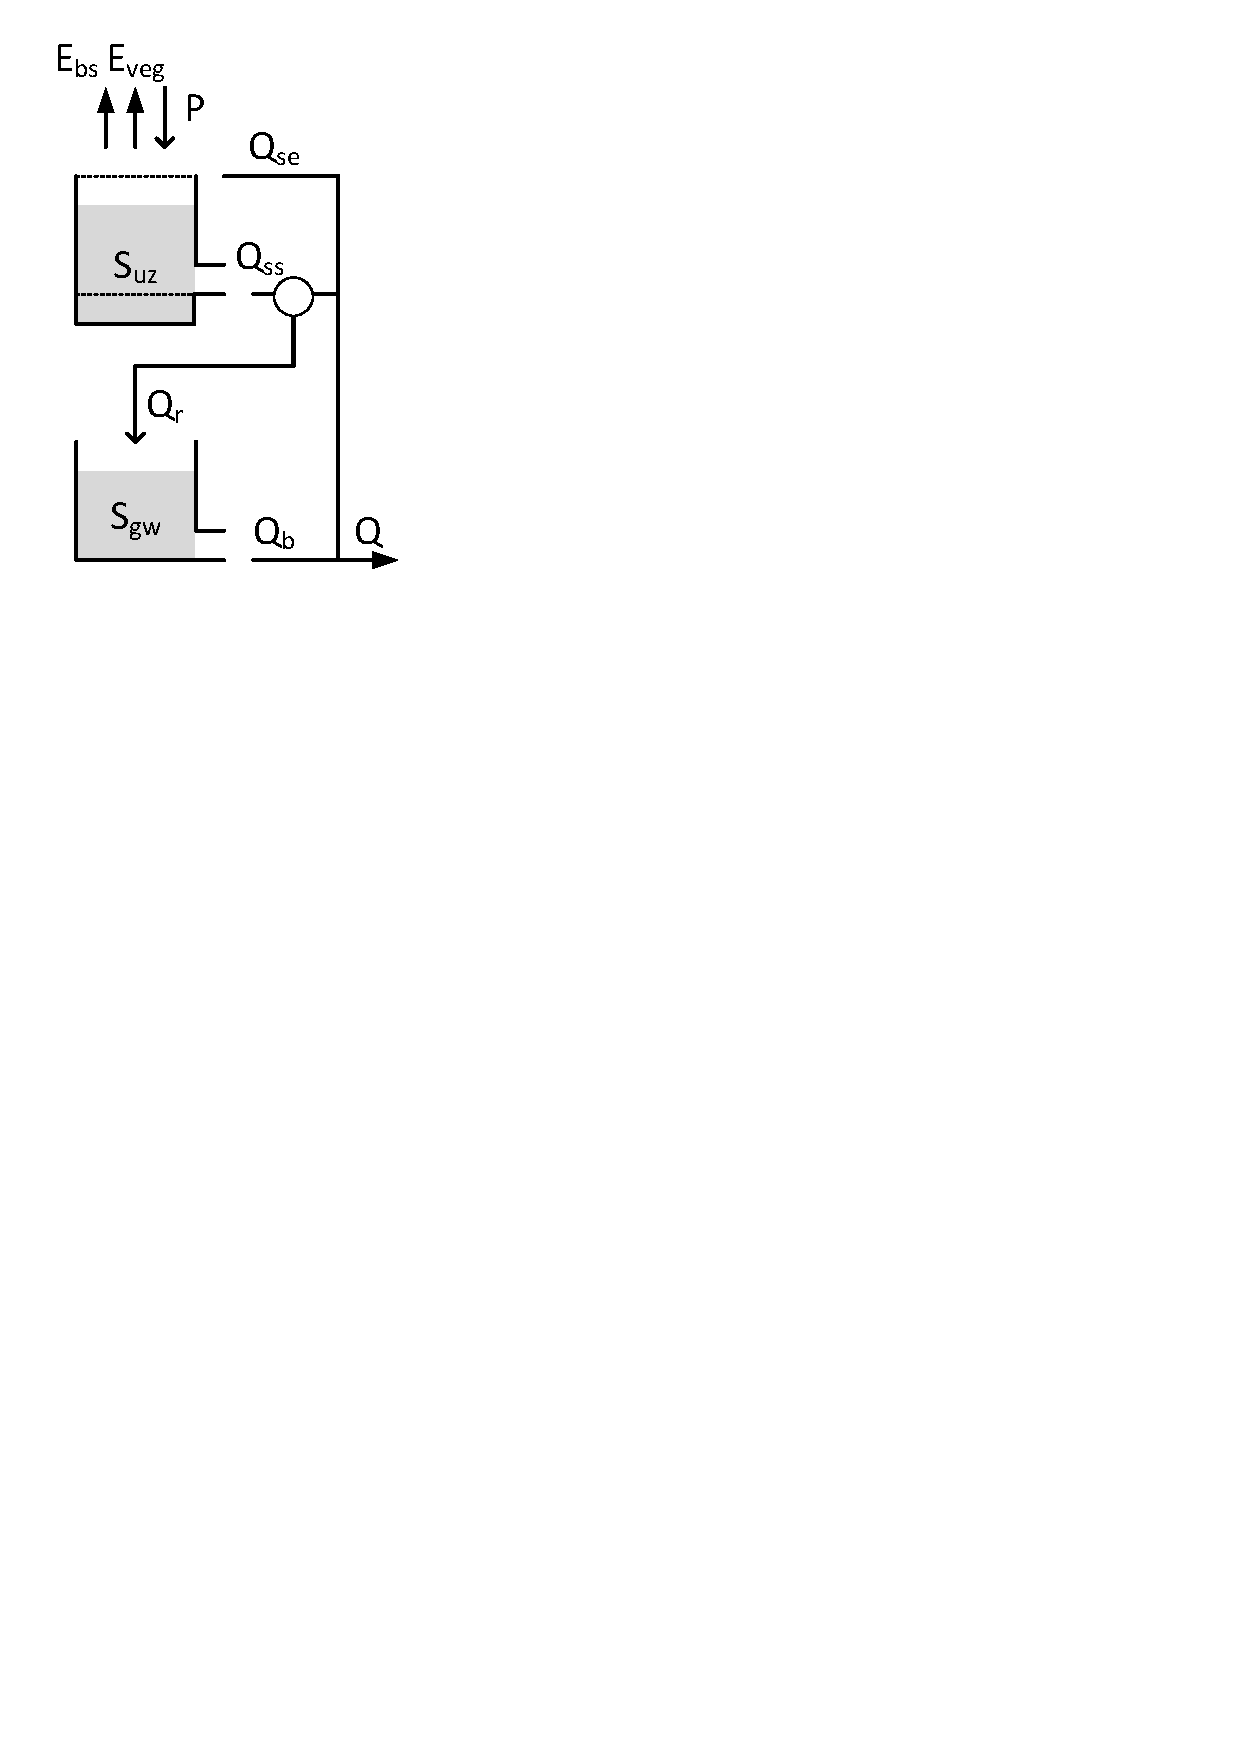
\includegraphics[trim=1cm 20cm 10cm 1cm,width=7cm,keepaspectratio]{./AppA_files/09_schematic.pdf}
\caption{Structure of the Susannah Brook model v1-5} \label{fig:09_schematic}
\end{wrapfigure}

\begin{align}
	\frac{dS_{uz}}{dt} &= P-E_{bs}-E_{veg}-Q_{se}-Q_{ss}\\
	E_{bs} &= \frac{S}{S_b}\left(1-M\right)E_p\\
	E_{veg} &= \begin{cases}
		M*E_p, &\text{if } S >S_{fc}\\
		\frac{S}{S_{fc}}M*E_p, &\text{otherwise}\\
	\end{cases}\\
	Q_{se} &= \begin{cases}
		P, &\text{if } S \geq S_b\\
		0, &\text{otherwise}\\
	\end{cases}\\
	Q_{ss} &= \begin{cases}
		\left(\frac{S-S_{fc}}{a}\right)^{\frac{1}{b}}, &\text{if } S > S_{fc}\\
		0, &\text{otherwise}\\
	\end{cases}
\end{align}

\vspace{2cm}
}

Where $S_{uz}$ is current storage in the upper zone [mm]. 
P [mm/d] is the precipitation input. 
$E_{bs}$ is bare soil evaporation [mm/d] based on soil depth 
$S_b$ [mm] and forest fraction $M$ [-]. $E_{veg}$ is transpiration from vegetation, using the wilting point $S_{fc}$ [mm] and forest fraction $M$. $Q_{se}$ is saturation excess flow [mm/d]. 
$Q_{ss}$ is non-linear subsurface flow, using the wilting point $S_{fc}$ [mm] as a threshold for flow generation and two flow parameters $a$ [d] and $b$ [-]. $Q_r$ is groundwater recharge [mm/d].

\begin{align}
	\frac{DS_{gw}}{dt} &= Q_r-Q_b\\
	Q_r &= r*Q_{ss}\\
	Q_b &= \left(\frac{1}{a}S_{gw}\right)^{\frac{1}{b}}
\end{align}	

Where $S_{gw}$ is the groundwater storage [mm], and $Q_b$ the baseflow flux [mm/d]. $r$ is the fraction of subsurface flow $Q_{ss}$ that goes to groundwater. Total flow [mm]:

\begin{align}
	Q &= Q_{se} + (Q_{ss} - Q_r) + Q_b
\end{align}

\subsection{Parameter overview}
% Table generated by Excel2LaTeX from sheet 'Sheet1'
\begin{table}[htbp]
  \centering
    \begin{tabular}{lll}
    \toprule
    Parameter & Unit  & Description \\
    \midrule
    $S_b$ & $mm$  & Maximum soil moisture storage \\
    $S_{fc}$ & $mm$  & Field capacity \\
    $M$   & $-$   & Forest fraction \\
    $a$   & $d$   & Runoff time coefficient \\
    $b$   & $-$   & Runoff nonlinearity \\
    $r$   & $-$   & Fraction subsurface flow to groundwater \\
    \bottomrule
    \end{tabular}%
  \label{tab:addlabel}%
\end{table}%


